\setcounter{section}{3}

\Needspace{5\baselineskip}
\hypertarget{modeling-touch}{%
\section{Modeling Touch}\label{modeling-touch}}

\Needspace{5\baselineskip}
\hypertarget{i.-challenges-of-tactile-modeling}{%
\subsection{I. Challenges of Tactile Modeling}\label{i.-challenges-of-tactile-modeling}}

\begin{enumerate}
\def\labelenumi{\arabic{enumi}.}
\item
  Lack of methods for obtaining large-scale tactile data. Effective tactile data available in industry is far scarcer than language or vision data. Tactile-equipped collection devices also retain high barriers to adoption, making collection difficult to scale.
\item
  Difficulty jointly modeling touch with language and vision. Touch usually occurs at the instant of robot--object contact and is high-frequency, while the signal may be absent at other times and thus sparse. Tactile data therefore cannot simply be mixed indiscriminately with language and vision.
\item
  Difficulty transferring across tactile sensors. Sensors include vision-based tactile, piezoresistive, capacitive, and other types, producing image, array, state, and other signal modalities at different resolutions, making general reuse difficult.
\item
  Different end-effector types have different sensor distributions. Grippers and dexterous hands, for example, differ in tactile-sensor placement and count, yet must operate through the same robot policy. This increases modeling difficulty, particularly for whole-body robot policies.
\end{enumerate}

\Needspace{5\baselineskip}
\hypertarget{ii.-main-approaches-to-tactile-modeling}{%
\subsection{II. Main Approaches to Tactile Modeling}\label{ii.-main-approaches-to-tactile-modeling}}

\Needspace{5\baselineskip}
\hypertarget{keeping-the-tactile-model-relatively-separate-from-the-main-policy}{%
\subsubsection{(1) Keeping the Tactile Model Relatively Separate from the Main Policy}\label{keeping-the-tactile-model-relatively-separate-from-the-main-policy}}

This approach makes touch an independent high-frequency correction module attached outside the main policy. For example, CraftNet divides a robot into three asynchronously operating components. System0 is an interaction loop running hundreds of times per second, specifically receiving force and torque signals and adjusting fingertip positions in real time at contact. Touch serves as the fastest correction loop.

\begin{figure}[htbp]
\centering
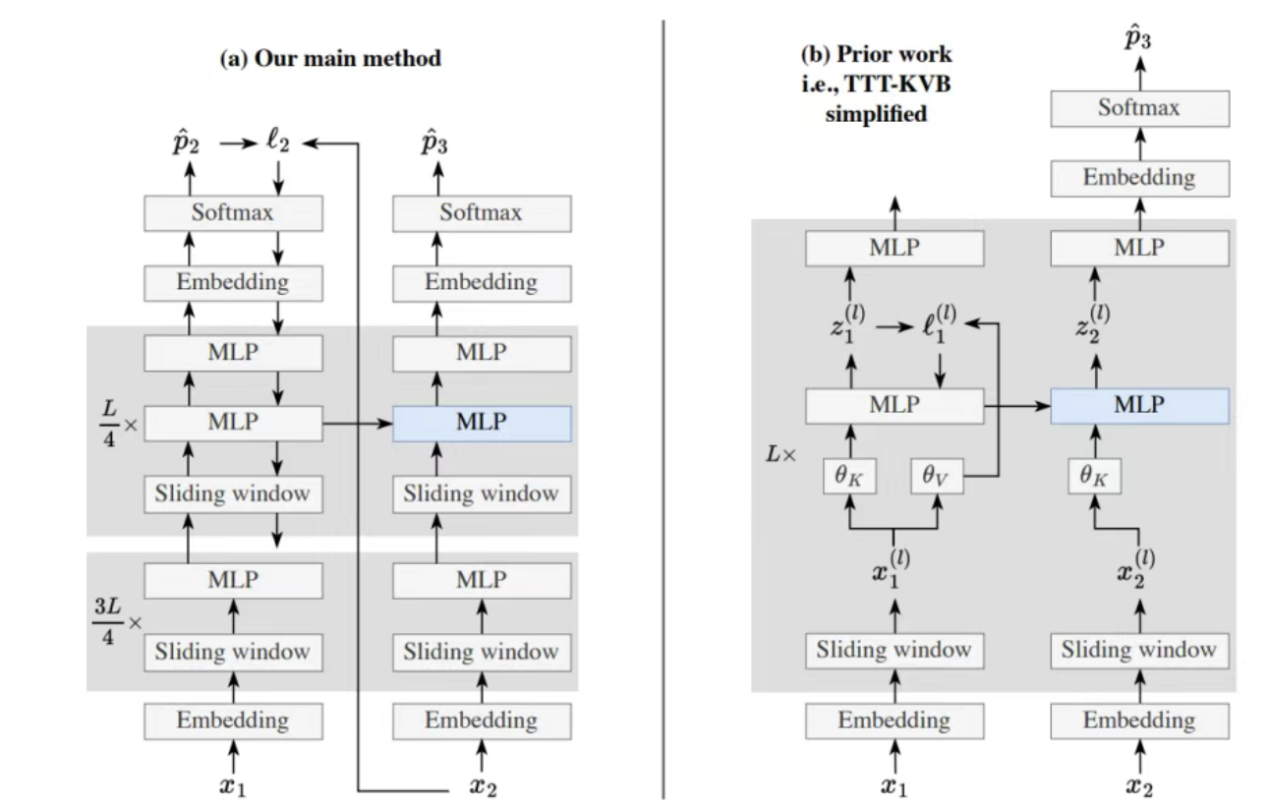
\includegraphics{images/image-0049.png}
\caption{CraftNet architecture separating the tactile model from the main policy}
\end{figure}

The drawback of this hierarchy is that touch does not enter backbone pretraining, limiting scaling potential compared with end-to-end unification and preventing cross-embodiment reuse.

\Needspace{5\baselineskip}
\hypertarget{connecting-to-the-main-policy-through-an-adapter}{%
\subsubsection{(2) Connecting to the Main Policy through an Adapter}\label{connecting-to-the-main-policy-through-an-adapter}}

Tactile-VLA, for example, uses an adapter to inject tactile tokens into a vision--language model, sharing attention with vision and language rather than building a separate system. Its advantage is that visual information can enter the main policy, achieving end-to-end unification and avoiding the inherent disadvantages of hierarchical architectures.

\begin{figure}[htbp]
\centering
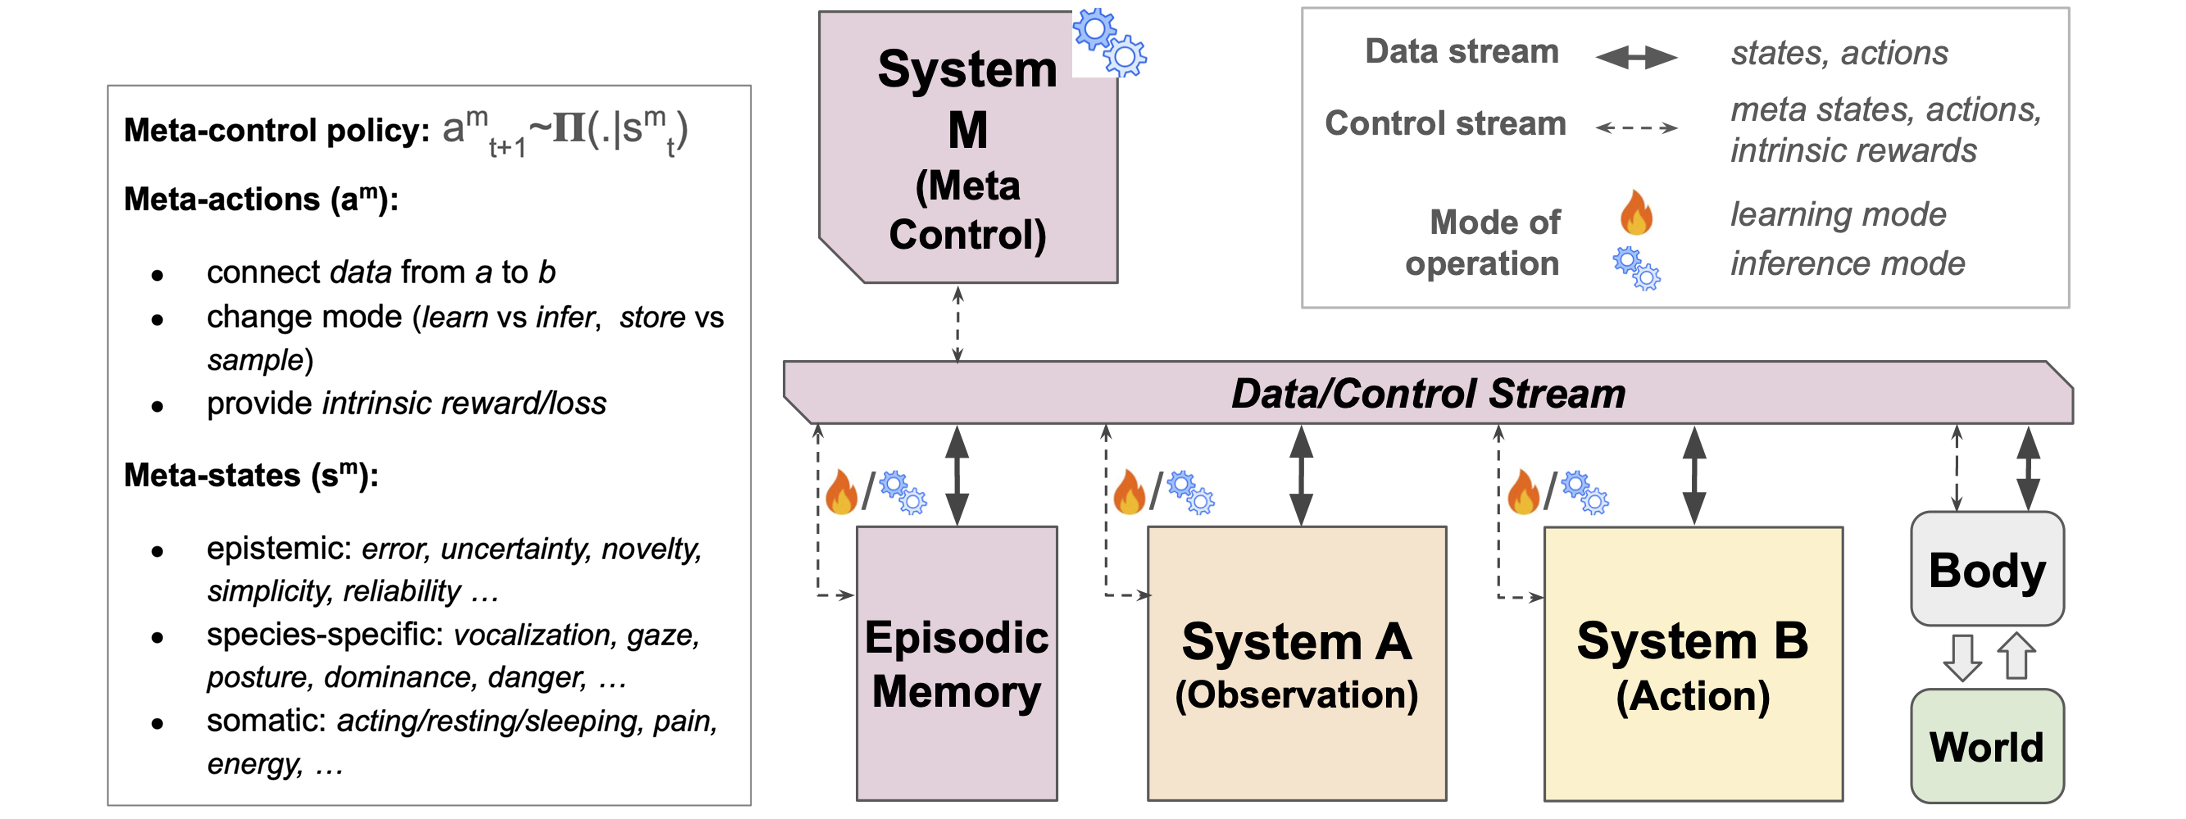
\includegraphics{images/image-0050.png}
\caption{Tactile-VLA architecture connecting to the main policy through an adapter}
\end{figure}

\Needspace{5\baselineskip}
Two drawbacks remain:

\begin{enumerate}
\def\labelenumi{\arabic{enumi}.}
\item
  When tactile information is later introduced to fine-tune an already trained vision--language model, touch and existing vision--language knowledge can interfere. Without proper modality fusion, forcibly combining touch with vision and language can not only fail to help but disrupt vision--language perception and harm overall performance.
\item
  The adapter remains tied to one sensor and cannot be reused after the sensor changes.
\end{enumerate}

\Needspace{5\baselineskip}
\hypertarget{separating-modalities-with-moe-inside-the-main-policy}{%
\subsubsection{(3) Separating Modalities with MoE inside the Main Policy}\label{separating-modalities-with-moe-inside-the-main-policy}}

A mixture of experts can use gating to control which expert dominates at different stages, relying mainly on vision without contact and sharply increasing tactile weight during contact. ForceVLA, for example, projects force readings into tokens and uses a force-aware MoE during action decoding for modality- and stage-aware routing. ForceVLA2 feeds forces into the VLM as text prompts to form ``force-aware task concepts,'' while also applying cross-scale MoE on the action side.

\Needspace{5\baselineskip}
MoE offers two benefits:

\begin{enumerate}
\def\labelenumi{\arabic{enumi}.}
\item
  Because touch differs substantially from vision and language, separating them through different weights avoids damaging pretrained vision--language knowledge.
\item
  Once the tactile-input format is defined, shared pretrained tactile experts can be reused during fine-tuning for previously unseen sensors. Only a lightweight encoder needs training to convert sensor data into a format readable by the tactile expert.
\end{enumerate}

\Needspace{5\baselineskip}
\hypertarget{iii.-ftp-1-a-foundation-model-incorporating-tactile-modeling}{%
\subsection{III. FTP-1: A Foundation Model Incorporating Tactile Modeling}\label{iii.-ftp-1-a-foundation-model-incorporating-tactile-modeling}}

\Needspace{5\baselineskip}
\hypertarget{specifying-the-tactile-sensor-data-format}{%
\subsubsection{(1) Specifying the Tactile-Sensor Data Format}\label{specifying-the-tactile-sensor-data-format}}

``FTP-1: A Generalist Foundation Tactile Policy Across Tactile Sensors for Contact-Rich Manipulation'' proposes the MTTS data interface. Its coordinates use the hand's functional regions, dividing each hand into 24 regions. Signals from any tactile sensor are assigned to these regions and translated into the same set of slot tokens. Each token has a functional-region embedding identifying where the sensation originates.

\Needspace{5\baselineskip}
\hypertarget{translating-different-sensor-signal-types}{%
\subsubsection{(2) Translating Different Sensor-Signal Types}\label{translating-different-sensor-signal-types}}

Image-based signals (deformation maps): Train a lightweight ViT to process images and convert them into MTTS-format tokens.

Array-based signals (pressure grids): Train a lightweight CNN to extract features and convert them into MTTS-format tokens.

State-based signals (force readings): Apply Fourier encoding, then train a lightweight MLP to transform the data format into MTTS-compatible tokens.

\Needspace{5\baselineskip}
\hypertarget{model-architecture-4}{%
\subsubsection{(3) Model Architecture}\label{model-architecture-4}}

\begin{figure}[htbp]
\centering
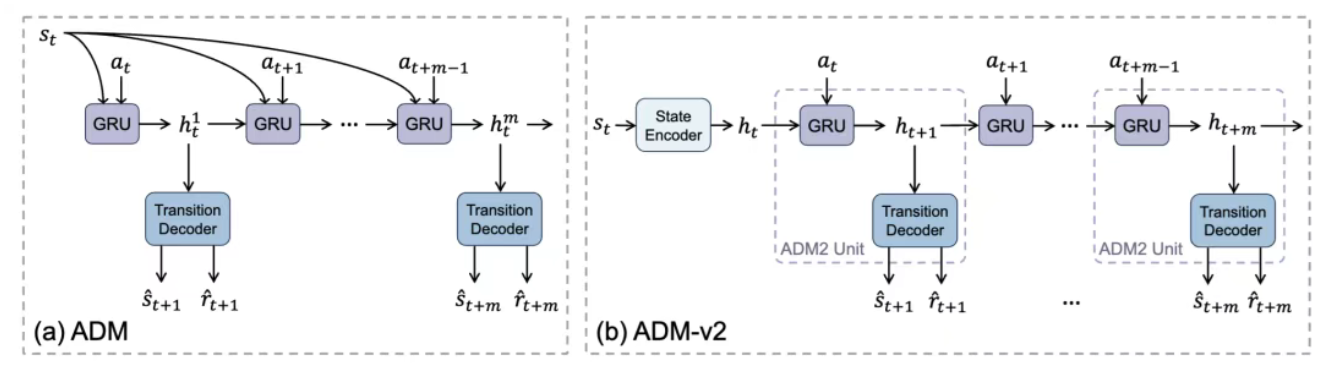
\includegraphics{images/image-0051.png}
\caption{FTP-1 tactile foundation-model architecture}
\end{figure}

After translation, different sensor signals enter the backbone, mainly composed of vision--language, action, and tactile experts. The vision--language expert has VLM capabilities, the action expert generates continuous actions through flow matching, and the tactile expert processes tactile signals. The action expert can obtain information unidirectionally from the tactile expert.

\FloatBarrier
\Needspace{5\baselineskip}
\hypertarget{references-161}{%
\subsection{References}\label{references-161}}

\vspace{0.25em}
\begin{itemize}
\tightlist
\item
  Sharpa. (2026). \href{https://www.sharpa.com/blogs/news/sharpa-announces-craftnet-a-hierarchical-vtla-model-for-fine-manipulation}{Sharpa Announces CraftNet: A Hierarchical VTLA Model for Fine Manipulation}. Official technical article.
\item
  Huang, J., Wang, S., Lin, F., Hu, Y., Wen, C., \& Gao, Y. (2025). \href{https://arxiv.org/abs/2507.09160}{Tactile-VLA: Unlocking Vision-Language-Action Model's Physical Knowledge for Tactile Generalization}. arXiv:2507.09160.
\item
  Yu, J., Liu, H., Yu, Q., et al.~(2025). \href{https://arxiv.org/abs/2505.22159}{ForceVLA: Enhancing VLA Models with a Force-aware MoE for Contact-rich Manipulation}. arXiv:2505.22159.
\item
  Li, Y., Zhaxizhuoma, Jiang, H., et al.~(2026). \href{https://arxiv.org/abs/2603.15169}{ForceVLA2: Unleashing Hybrid Force-Position Control with Force Awareness for Contact-Rich Manipulation}. arXiv:2603.15169.
\item
  Yuan, C., Zhang, Z., Zhou, M., et al.~(2026). \href{https://arxiv.org/abs/2606.13102}{FTP-1: A Generalist Foundation Tactile Policy Across Tactile Sensors for Contact-Rich Manipulation}. arXiv:2606.13102.
\item
  具身纪元. (2026). \href{https://www.jintiankansha.com/t/DWG4NegaMt}{Touch Needs Its Own Foundation Model and Open-X Embodiment} (translated title; in Chinese). WeChat public-account article.
\end{itemize}

\clearpage
